\documentclass[a4paper, amsfonts, amssymb, amsmath, reprint, showkeys, nofootinbib, twoside]{revtex4-1}
\usepackage[spanish]{babel}
\usepackage[utf8]{inputenc}
\usepackage{float}
\usepackage[colorinlistoftodos, color=green!40, prependcaption]{todonotes}
\usepackage{amsthm}
\usepackage{mathtools}
\usepackage{physics}
\usepackage{xcolor}
\usepackage{graphicx}
\usepackage[left=23mm,right=13mm,top=35mm,columnsep=15pt]{geometry} 
\usepackage{adjustbox}
\usepackage{placeins}
\usepackage[T1]{fontenc}
\usepackage{lipsum}
\usepackage{csquotes}
\usepackage[normalem]{ulem}
\useunder{\uline}{\ul}{}
\usepackage[pdftex, pdftitle={Article}, pdfauthor={Author}]{hyperref} % For hyperlinks in the PDF
%\setlength{\marginparwidth}{2.5cm}
\bibliographystyle{apsrev4-1}

\begin{document}

%El título del experimento realizado es importante.
\title{Bernoulli}


\author{Sergio Montoya}

%Si necesitan poner un segundo autor, deben eliminar los porcentajes (%) iniciales.
  
\author{Carlos Devia}

\affiliation{Universidad de los Andes, Bogotá, Colombia.}

\date{\today} % Si lo dejan vacío no les saldrá fecha. La fecha que se muestra es del día en que se compila.

\maketitle

\section{Análisis Cuantitativo}

\begin{enumerate}
  \item Si por un tubo está fluyendo agua y luego el radio del
tubo se reduce, ¿qué pasa con la rapidez del agua?
¿Qué pasaría con la rapidez si el tubo no solo redujera
su radio sino que aumentara su altura? ¿Qué pasaría
también con la presión en ambos casos?

\textbf{Solución:}

En el primer caso, se da que el fluido viajaría mas rápido. Esto de hecho podríamos encontrarlo desde la ecuación $12.7$. Pues en este caso ocurriría un cambio en la presión (Cosa clara, puesto que estamos alterando el volumen y inconsecuencia el  área en el que se aplica la fuerza) y por tanto otro valor debería cambiar y dado que en este caso no estamos haciendo que la altura cambie entonces la rapidez debería aumentar. En el segundo caso  por un análisis similar de la ecuación  $12.7$ podemos notar que el fluido no tendría por que acelerar y dependería entre la relación de altura nueva y presión lo que marcaría el cambio de este. Siendo la disminución de su radio un aporte a su velocidad y la altura una contraria.

\item Si se tienen dos hojas delgadas de papel muy cercanas
a ellas y se sopla entre ellas estas se unen. ¿Cómo puede explicar esto? ¿Qué tiene que ver con el principio
de Bernoulli en esta situación?

\textbf{Solución:}

Si usted sopla hace que la velocidad del fluido entre ellas aumente y  en consecuencia dado que se mantiene la misma altura y por la ecuación $12.7$ tendría que cambiar su presión. En particular esta tendría que disminuir (Dado que la velocidad aumenta) y por tanto esto lo experimentarían las hojas como una fuerza que las hace unirse.


\item “La ecuación de Bernoulli nos dice que, donde la rapidez del fluido es más alta, la presión es más baja,
y viceversa”. ¿Esta afirmación es siempre válida? Explique.

\textbf{Solución:}

No siempre es valida. Es muy importante tomar en consideración la altura, la densidad y la viscosidad del fluido. Aunque estas variables si que están relacionadas por el principio de Bernoulli no tiene por que ser tan directa la consecuencia.

\item  ¿Por qué las chimeneas se construyen tan altas? Argumente.

  \textbf{Solución:}
  Posiblemente para hacer que la presión y velocidad no sean tan altas. Es una manera de encontrar balance.
\end{enumerate}

\section{Análisis Cualitativo}

\textbf{Con $H$ constante}

En este caso, se esperaba ver una gráfica de modo tal que al aumentar  $y$ se aumentara tambien la distancia recorrida. Esto se desarrollo mejor en la sección de Teoría de la guía. De hecho, la conclusión principal de esta sección en la guia consiste en llegar a este resultado. Para hacerlo hacen un análisis de fuerzas para una partícula de este flujo.

Ahora bien, aunque los datos tomados no fueron suficientes se le pidieron los datos a unos compañeros con lo que podemos obtener las siguientes gráficas:

 \begin{figure}[htpb]
  \centering
  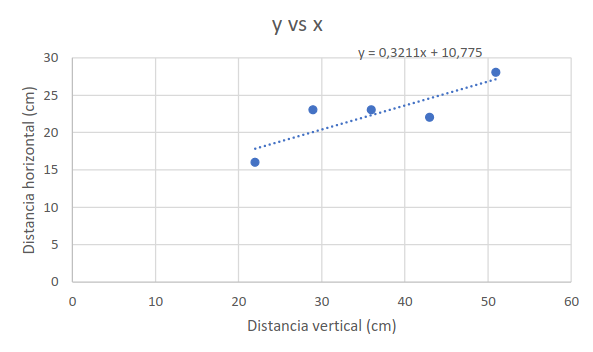
\includegraphics[width=0.4\textwidth]{yvsx.png}
  \caption{Gráfica de como varia la posición en el eje $x$ al hacer que el agua caiga de una mayor altura.}
  \label{fig:yvsx}
\end{figure}

Con esta podemos utilizar la ecuación $12.12$ y encontrar los tiempos en el aire los cuales fueron de

 \begin{table}[htpb]
  \centering
  \caption{Tabla de los tiempos en el aire para una partícula que cae en el fluido en función de $y$} 
  \label{tab:label}
  \begin{tabular}{|c|c|} 
    \hline
    $y$ & tiempo \\
    51 & 0,32 \\
    43 & 0,39 \\
    36 & 0,27 \\
    29 & 0,24 \\
    22 & 0,21  \\
    \hline
  \end{tabular}
\end{table}

\textbf{Con $Y$ Constante}

Una vez mas se esperaría obtener un resultado directamente proporcional. Este también se da por la ecuación  $12.14$  y una vez mas con la ayuda de nuestros compañeros podemos adjuntar esta gráfica:

\begin{figure}[htpb]
  \centering
  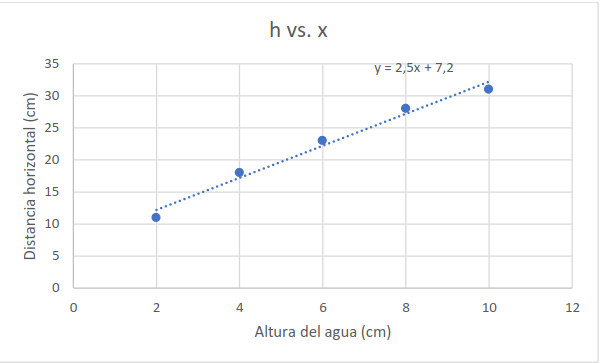
\includegraphics[width=0.4\textwidth]{hvsx.png}
  \caption{Gráfica de la distancia en función de $h$}
  \label{fig:hvsx}

  La cual nos muestra lo que esperábamos.
\end{figure}


\section{Conclusiones}

Para este experimento se esperaba lograr entender Bernoulli. Este es un efecto que lo que hace es esencia relacionar la presión con la velocidad y la altura. Aun así, es de mencionar que no se lograron los objetivos prácticos por falta de datos. Esto tiene como consecuencia que se logro un entendimiento teórico de este efecto pero no se consiguieron los objetivos planteados para el laboratorio. Ahora bien, con ayuda de nuestros compañeros que si nos dieron los datos pudimos notar que estos correspondían con lo esperable por la teoría. Por lo tanto aunque no fue con nuestros propios datos si se consiguió mostrar el teorema de Bernoulli funciona para flujo estacionario.

\end{document}
